\documentclass[13pt]{article}
%Gummi|065|=)
\title{\textbf{CIRCUITOS DE ACTIVACIÓN CON TRANSISTORES}}
\author{Guzmán Vázquez Jaime Alan Yamil.\\UPZMG\\SISTEMAS ELECTRÓNICOS DE INTERFAZ.}
\date{29 octubre }
\usepackage{graphicx}
\begin{document}
\begin{figure}[htp]
\centering

\includegraphics[scale=1.00]{/home/emile/Escritorio/guzman.vazquez.jaime.alan.yamil/tareas/EV_2_8_CALCULAR_LOS_PARAMETROS_DE_CIRCUITOS_DE_ACTIVACION_DE_TRANSISTORES_DE_POTENCIA./imagenes/índice.png}
\caption{}
\label{}
\end{figure}
\maketitle

\section{CONTEXTO}
Para poner un poco en contexto y saber porque se realizan estos cálculos se necesita definir primeramente que es un transistor, en el apartado de cálculos se mostrara un ejemplo sobre la cuestión practica de estos cálculos.\\\\

TRANSISTOR\\
primeramentte definiremos que es un transistor y cual es su método de uso, el transistor se podria interpretar como una compuerta AND el programacion pero de manera electronica, este nesecita de dos fuentes de voltaje corriendo por dos de sus patas para poder dejar fluir el voltaje por la tercera, las configuraciones que pueden ser utiliazadas mas comunmente es la PNP Y NPN, a continuacion se mostrara una imagen tanto de la forma en la que esta construida asi como su encapsulado.\\
\begin{figure}[htp]
\centering
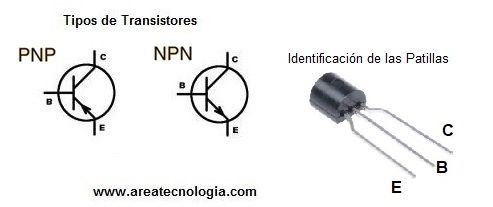
\includegraphics[scale=0.50]{/home/emile/Escritorio/guzman.vazquez.jaime.alan.yamil/tareas/EV_2_8_CALCULAR_LOS_PARAMETROS_DE_CIRCUITOS_DE_ACTIVACION_DE_TRANSISTORES_DE_POTENCIA./imagenes/tipos-transistores.jpg}
\caption{}
\label{}
\end{figure}\\\\



\section{CALCULOS}
Los cálculos que se realizaran a continuación son básicamente los parámetros comunes que se necesitan saber de un circuito, ya sea la resistencia en cada uno de los lugares del circuito, el voltaje necesario para encender el dispositivo o componente que se desea utilizar y la corriente que se requiere en el circuito.\\\\
Ejemplificaremos los cálculos con una aplicacion de un LED necesita un amperaje que no puede ser suministrado por una placa de control común.\\
\\
Tenemos un micro controlador que tiene 5 voltios como mayor tensión y un amperaje máximo de 10mA y un led que necesita 1.7 voltios y 8mA, necesitariamos calcular el valor de la resistecia que se podria entre el controlador y el led, se utilizara ley de kirtchoff para calcular el voltaje de la resistencia dada de la siguiente manera:\\\\

$$Vr=Vout-Vled$$\\
donde Vr es voltaje en la resistencia\\
Vout es voltaje en el microcontrolador\\
Vled seria la tensión necesaria para el led\\
\\
esto se resta  debido a que todo lo que no aporte carga la resta de la ya existente.\\
con nuestros datos quedaría:\\

$$Vr=5v-1.7v=3.3v$$\\\\
Para calcular la resistencia del circuito realizaremos los cálculos en base a la ley de Ohm donde:\\
$$V=I*R$$\\
despejando:\\
$$R=\frac{V}{I}$$\\
ajustando a nuestras variables:\\
$$R=\frac{Vr}{IT}$$\\
$$R=\frac{3.3v}{8mA}=412.5 ohm$$\\
*Se utilizara el valor comercial de 470 ohm puesto a que la corriente baja en el circuito en vez de aumentar con esto, lo que lo hace mas seguro, con esto quedarían 7mA al final.\\\\
Al necesitar usar un LED con mayor potencia que sus datos serian 3.6v y 100mA de consumo es cuando la verdadera aplicacion del transistor se deja ver, se utilizara el TIP 41 con transistor para ejemplificar.\\
Se usara la formula:\\
$$Ic=hFE*Ib$$\\
donde Ic es la corriente en el colector\\
Ib es la corriente en la base \\
y hFE seria el valor de multiplicación del transistor(se encuentra en datasheet o con multímetro.)\\\\
se tendra el colector ocupado por la fuente de voltaje para el LED, el LED junto con su resistencia, para la base se tendra la placa de control y en el emisor la tierra.\\
Para calcular la resistencia del LED seria la siguiente expresion:\\
$$RL=\frac{5v-3.6v-0.3v}{100mA}=11 omh$$\\
Para la intensidad de la base seria la siguiente formula:\\
$$Ib=\frac{Ic}{hFE}$$\\
$$Ib=\frac{100mA}{75}=1.3mA$$\\
Los mismos calculos son realizados para la parte de la base del transistor teniendo:\\
$$Rb=\frac{5v-0,7v}{1.3mA}=3307 ohm$$\\
Estos serian todos los calculos necesarios para realizar esta configuracion del transistor.\\

\section{USOS}
comprender mejor el tema de este tipo de cálculos y sus aportaciones al mundo de la electrónica es necesario hablar sobre algunos aspectos en los que podría ayudar este tipo de configuraciones en circuitos con diferentes limitaciones mayormente de potencia.\\\\
Un ejemplo muy resaltaste que se puede observar en la electrónica es poder conservar los mejores aspectos de la electrónica de potencia así como las grandes cantidades de tensión que se soportan o el poder controlar diferentes dispositivos de gran poder y tamaño con componentes especializados y la forma de control que tiene la electrónica digital como lo podrían ser placas de control como arduino o raspberry o componentes integrados con su efectividad, gran resistencia al ruido y fiabilidad, ademas de su gran gama de posibilidades.\\\\
Juntar estos dos tipos de electrónica es algo imprescindible y el uso del transistor como switch que interfiera en estos es muy importante, aplicaciones que se podrían dar con este tipo de configuraciones podrían ser el manipular un motor de gran potencia con una placa de control con activador que permita el paso de la tensión que necesita mientras que el circuito solamente es completado o manipulado por la electrónica digital que permite el paso de la energia de potencia.\\\\
Esta podría ser una de las muchas aplicaciones que esta configuración podría tener en funcion de lo que necesite.\\\\

\section{referencias}
youtube/electgpl Electronica.\\
Incb.com.mx\\
sistemasorp.es\\



\end{document}
